\section{Projektverwaltungswerkzeuge}
Der Einsatz von Projektverwaltungswerkzeugen in der Softwareentwicklung hat das Ziel, die Verwaltung und das Projektmanagement zu vereinfachen und zu unterstützen. Des Weiteren sollen die Anwendungen die Entwickler bei der Verwaltung ihrer Projektaufgaben entlasten und die Produktivität steigern.\\

\subsection{Anforderungen}\label{ssec:anforderungen}
Die Anforderungen an ein Projektverwaltungswerkzeug unterscheiden sich je nach Projektkomplexität und Anzahl der Teilnehmer. Grundsätzlich gilt, je größer die Anzahl der Teilnehmer, desto ratsamer ist eine software-gestützte Verwaltung einzusetzen.
Das Projektverwaltungswerkzeug für die agile Softwareentwicklung muss dabei die gängigen agilen Projektverwaltungsaufgaben unterstützen. Diese funktionalen Anforderungen sehen wie folgt aus:

\begin{description}
	\item[Ressourcenverwaltung]\hspace*{1em}\\
Die Ressourcenverwaltung des Projekts erlaubt die Überwachung und Planung von Ressourcen wie die Kapazität von Mitarbeitern, das Budget und den Zeitaufwand.
	\item[Rollenverteilung]\hspace*{1em}\\
Die Rollenverteilung bestimmt die Rolle jedes Mitarbeiters in einem Projekt.
	\item[Zeitverwaltung]\hspace*{1em}\\
Diese Anforderung erlaubt die Analyse von Zeitaufwänden von Stories/Tasks.
	\item[Aufgabenverteilung]\hspace*{1em}\\
Die Aufgabenverteilung regelt die Auswahl der zu bearbeitenden Stories/Tasks, die von den Entwicklern eigenständig ausgewählt werden können.
	\item[Problemmanagement]\hspace*{1em}\\
Das Problemmanagement dient zum Erfassen von Korrekturvorschlägen und die Meldung von Fehlverhalten in bereits erstellter Software. 
	\item[Releaseplanung]\hspace*{1em}\\
Die Vergabe von festen Termine für den Release von bestimmten Softwareständen zu planen.\\
\end{description}
Des Weiteren unterliegt das Projektverwaltungswerkzeug allgemeinen Software Anforderungen. Mit diesen nicht-funktionalen Anforderungen lässt sich das passende Produkt für den Produktiveinsatz ermitteln.

\begin{description}
	\item[Benutzbarkeit]\hspace*{1em}\\
Die Benutzbarkeit ist die Bedienfreundichkeit einer Anwendung. Diese Anforderung zeigt, wie leicht man eine graphische Oberfläche bedienen kann, wie übersichtlich und wie intuitiv sich diese Bedienen lässt.
	\item[Effizienz]\hspace*{1em}\\
Die Effizienz zeigt an wie hoch der Ressourcenverbrauch der Software ist. Zu den wichtigen Ressourcen gehören der Speicher- und die CPU-Auslastung.
	\item[Wartbarkeit]\hspace*{1em}\\
Die Anforderung der Wartbarkeit beschriebt die Möglichkeit das System durch beispielsweise Korrekturen oder Anpassungen zu ändern.
	\item[Portierbarkeit]\hspace*{1em}\\
Die Portierbarkeit einer Software sagt aus, wie leicht sich eine Software auf andere Systeme portieren lässt, ob andere Systeme unterstützt werden oder die Software austauschbar ist.
	\item[Zuverlässigkeit]\hspace*{1em}\\
Die Zuverlässigkeit der Software zeigt die Fehlertoleranz gegenüber Eingaben, das Wiederherstellen bei Abstürzen und eine konsistente Datenhaltung. 
	\item[Lizenzierung]\hspace*{1em}\\
Diese Anforderung bezieht sich auf die rechtliche Verwendungslage von Software. Darin werden der Einsatz und die Verbreitung der Software geregelt.
	\item[Skalierbarkeit]\hspace*{1em}\\
Die Skalierbarkeit bezieht sich auf die Anzahl der Benutzer und der Anzahl der zu verwaltenden Projekte.
\end{description}

\subsection{Propriet"are Software}
Aufgrund einer Vielzahl an verschiedenen Projektverwaltungsapplikationen werden in diesem Unterpunkt nur Applikationen, die speziell für den agilen Einsatz beworben werden, vorgestellt.

\begin{description}
\item[in-Step Scrum Edition]\hspace*{1em}\\
Das Projektverwaltungswerkzeug \emph{in-Step Scrum Edition} wird von dem Unternehmen \emph{microTOOL} angeboten. Dieses Werkzeug ist in verschiedene Komponenten aufgeteilt. Für den Einsatz dieser Projektverwaltung muss ein \emph{in-Step Server} eingerichtet werden. Dieser Server kann mittels \emph{in-Step Windows Clients}, die auf den entsprechenden \emph{Windows} Rechnern installiert werden müssen, benutzt werden. Zusätzlich wird noch ein \emph{in-Step Web Client} angeboten, der eine Bedienung über den Webbrowser zulässt. \emph{in-Step Scrum Edition} ist eine spezielle Variante, welche für die agile Vorgehensweise \emph{Scrum} vorgesehen ist. Dabei wird das Projektmanagement durch folgende Punkte unterstützt:
\begin{itemize}
\item Projektanforderungsverwaltung\\
Die Projektanforderungsverwaltung hilft dabei, dass Projektanforderungen in eine User Story überführt werden. Dabei wird jede Story versioniert und eine Historie angelegt. Dadurch können Änderungen im Projektverlauf nachvollzogen werden. Für jede User Story kann eine Priorität, ein geschätzter Aufwand und ein Geschäftswert eingetragen werden.

\item Sprit-Planung\\
Sprints werden in \emph{in-Step Scrum Edition} als Balken entlang einer Zeitachse dargestellt. Für den Sprint werden aus User-Stories Tasks abgeleitet, die dabei versioniert werden. Die Tasks erscheinen in einer editierbaren Liste, die den aktuellen Zustand und den Restaufwand des Tasks anzeigen. Neue Tasks werden zudem noch auf die integrierte Team Anzeigetafel gestellt.

\item Release-Planung\\
Ein Release wird in einem Zeitdiagramm nach einem oder mehreren Sprints als Meilenstein eingetragen. Dabei kann bestimmt werden, welche User Story in den Release kommt, anhand der Priorität der User Story. Die Stories können dadurch automatisch an Releases zugewiesen werden. 

\item Projektüberwachung\\
Durch Burndown Charts kann die Entwicklung für den aktuellen Sprint oder den kommenden Release überwacht werden. Diese werden als Linien- oder Balkendiagramm mit zusätzlichen Infos, wie zum Beispiel Restaufwand, Ist-Aufwand und einer Prognose für den weiteren Verlauf, visualisiert.

\item Produktverwaltung\\
Mit Hilfe einer zentralen Produktbibliothek lassen sich alle Projektergebnisse archivieren und verwalten. Dadurch ist es möglich aktuelle Produktstände zu ermitteln und herauszufinden, welche Versionen verschiedener Produkte einen gemeinsamen Entwicklungsstand repräsentieren.

\end{itemize}

Die Entwickler werden durch eine integrierte Anzeigetafel mit den aktuellen Projektinformationen versorgt. Diese Anzeigetafel ist in Spalten, die Zustände repräsentieren, unterteilt. Die Tasks durchlaufen dabei die verschiedenen Spalten, bis sie von den Entwicklern abgearbeitet sind. Des Weiteren gibt es Integrationen in die Entwicklungsumgebungen \emph{Eclipse} und \emph{Microsofts Visual Studio}, die Verarbeitung der Tasks vereinfachen. \cite {bib:instep} \\

%\item[Rally]\hspace*{1em}\\
%eventuell weglassen; je nach Umfang der anderen Produkte

\item[TargetProcess]\hspace*{1em}\\
Die Projektverwaltungssoftware \emph{TargetProcess} unterstützt die die agilen Vorgehensweisen \emph{Scrum}, und \emph{Extreme Programming}. Dabei ist \emph{TargetProcess} eine Serveranwendung, welche über einen Webbrowser bedient wird. Der Zugang kann dementsprechend für die Intranet- oder Internetnutzung freigegeben werden.
Die Anwendung unterstützt das Projektmanagement durch folgende Funktionen:
\begin{itemize}
\item Iterationen planen\\
Beim Planen der Iterationen kann eine Priorisierung von User Stories oder Bugs vorgenommen werden. Die User Stories für die nächste Iteration kann ebenfalls ausgewählt werden.

\item Taskboard\\
Tägliche Besprechungen können auf dem Taskboard festgehalten werden. Dadurch kann jedes Teammitglied auf dem aktuellen Informationsstand gehalten werden. Im Taskboard werden ebenfalls neu angelegte Tasks oder Statusänderungen von Tasks angezeigt.

\item Entwicklungsprozesse Überwachen und Visualisieren\\
Die bereits abgearbeiteten User Stories können in Zeitdiagrammen angezeigt werden. Des Weiteren lassen sich eventuelle Verzüge oder die Geschwindigkeit der einzelnen Teams in einem Burn Down Diagramm visualisieren. Durch eine Ablauftabelle lässt sich der tägliche Verlauf von Tasks überwachen und eventuell kritische Tasks lokalisieren.

\item Release Planung\\
Die Planung der verschiedenen Releases lässt sich in in einem interaktiven Diagramm vornehmen. Dabei können eventuelle Verzögerungen eines Releases anhand von kritischen Tasks angezeigt werden.

\item Zeitplanung\\
Der Zeitaufwand jedes einzelnen Tasks kann angezeigt werden. Dabei kann der geplante Zeitaufwand mit dem tatsächlichen verglichen werden.
\end{itemize}

\emph{TargetProcess} bietet aber nicht nur Funktionen für den Projektleiter/Scrum Master, sondern auch für die einzelnen Entwickler des Projekts. Die Entwickler werden bei ihrer Arbeit durch folgende Funktionen des \emph{TargetProcess} unterstützt:
\begin{itemize}
\item Task Bearbeitung\\
Die Auswahl eines Tasks kann leicht vorgenommen werden. Dabei können Prioritäten von Tasks die Auswahlmöglichkeiten an abzuarbeitenden Tasks anpassen. Dadurch können die einzelnen Entwickler sich die Tasks aussuchen, welche sie in der Iteration abarbeiten.

\item Integration in Entwicklungsumgebungen\\
Durch Plug-Ins oder Add-Ins in Entwicklungsumgebungen wie \emph{Microsofts Visual Studio 2011} werden Verwaltungsaufgaben vereinfacht. So können Bugfixes direkt über die Entwicklungsumgebung an das \emph{TargetProcess} System mitgeteilt werden.

\item Zeitplanung\\
Die aufgewendete Zeit für einen Task wird protokolliert und der tägliche Arbeitsaufwand kann ausgewertet werden.
\end{itemize}

Zusätzlich zu den oben genannten Funktionen des Systems unterstützt \emph{TargetProcess} auch die Qualitätssicherung eines Projekts. Dies wird mit folgenden Funktionen möglich:
\begin{itemize}
\item Testcase Ergebnisse pro Iteration/Release/Build darstellbar
\item Bug Report mit neu hinzugekommenen, gelösten und bestehenden Fehlern
\end{itemize}

Abgerundet wird der Funktionsumfang durch die Möglichkeit Kundenwünsche erfassen zu können und in entsprechende Tasks zu formen. Dabei können auch die einzelnen Anforderungen an das Produkt verwaltet und kategorisiert werden. \cite{bib:targetprocess} \\

\item[Team Foundation Server 2010]\hspace*{1em}\\
Der \emph{Team Foundation Server 2010} des Softwareunternehmens \emph{Microsoft} ist eine Komplettanwendung zum Erstellen und Verwalten von Software-Projekten. Dabei unterstützt der \emph{Team Foundation Server} agile Vorgehensweisen wie beispielsweise \emph{Scrum} durch vorgefertigte Vorlagen für andere \emph{Microsoft} Produkte. Es werden folgende Vorlagen für das agile Projektmanagement mitgeliefert:
\begin{itemize}
\item Planung von Iterationen\\
Die Iterationsplanung erfolgt mit Hilfe von \emph{Microsoft Excel} Arbeitsmappen. In diesen Arbeitsmappen werden die entsprechenden Tasks für die anstehende Iteration geplant und eingetragen. Bei Änderungen aktualisiert der \emph{Team Foundation Server 2010} diese Tabellen. Über den \emph{TFS 2010} können dann die Entwickler die Tasks zur Bearbeitung annehmen.

\item Projektanforderungsverwaltung\\
Für die Projektanforderungsverwaltung wird eine \emph{Microsoft Excel} Vorlage bereitgestellt, die eine Kapazitätsplanung auf Basis von vorherigen Iterationen erlaubt.

\item Entwicklungsprozessüberwachung\\
Der Entwicklungsprozess kann leicht durch Burndown Berichte überwacht werden.

\item Portfolioverwaltung\\
Durch Vorlagen für \emph{Microsoft Excel} und \emph{Project} bekommen Abteilungsleiter und Projektmanager detaillierte Einblicke in aktuelle Projekte und können kontrollieren, wie die Projekte die Anforderungen des Unternehmens unterstützen.

\end{itemize}

Die Unterstützung der Arbeit für Entwickler ist durch ein integriertes Datawarehouse sehr hoch. In diesem Datawarehouse wird die Aufgabenverwaltung, der Quellcode, die Builds und die Testwerkzeuge gespeichert. Des Weiteren ist die Unterstützung des \emph{Team Foundation Server 2010} in der Entwicklungsumgebung \emph{Visual Studio 2010} bereits integriert. \cite{bib:tfs2010} \cite{bib:tfsheise} \\

\end{description}

\subsection{Open-Source Software}
Im Open-Source Bereich findet sich auch eine Vielzahl an Projektverwaltungssoftware zur Unterstützung bei der agilen Vorgehensweise. Deshalb wird in diesem Unterpunkt nur ein Teil an Projekten vorgestellt, die weiter aktiv von der Community weiterentwickelt werden. Der Vorteil an Open Source Software liegt hier in der möglichen Mitbestimmung der künftigen Entwicklung durch Beteiligung in der Community oder durch eine Überarbeitung und Anpassung des Projekts an die eigenen Strukturen, Gegebenheiten und Prozesse.
\begin{description}
\item[Agilefant]\hspace*{1em}\\
Das Projekt \emph{Agilefant} ist eine webbasierende Serveranwendung, die in der Programmiersprachen Java entwickelt wird. Dabei werden keine speziellen agilen Vorgehensweisen unterstützt, sondern allgemein die agile Projektverwaltung.
\begin{itemize}
\item Produktmanagement\\
Das Produktmanagement ermöglicht die Planung von Produkten, die in mehrere Release Projekte aufgeteilt sein können. Dabei kann die Produktgeschichte hierarchisch angezeigt werden.
\item Release Planung\\
Die Planung von Releases für Projekte kann anhand von festen Zeitvorgaben vorgenommen werden. An diese Projekte sind Stories geknüpft, welche abgearbeitet werden. Durch den Abarbeitungsstatus der einzelnen Stories kann eine Überwachung des Releasedatums erfolgen und eventuell kritische Stories aufzeigen.
\item Iterationen\\
Die Stories können in Tasks mit Prioritäten aufgeteilt werden. Die einzelnen Tasks könne dann von Entwicklern abgearbeitet werden.
\item Zeitmanagement\\
\emph{Agilefant} kann den Aufwand von Aufträgen, Stories und einzelnen Tasks aufzeichnen. Diesen Aufwand kann als Webreport oder Excel Tabellenkalkulation ausgegeben werden.
\item Entwicklungsprozesse Überwachen und Visualisieren\\
Der Entwicklungsprozess eines Projekts lässt sich mit Hilfe von verschiedenen Diagrammen visualisieren. In diesen Diagrammen werden die Zustände von Tasks, Iterationen und Stories bewertet und in einer zeitlichen Listung dargestellt. 
\item Portfolio Verwaltung\\
Alle aktuellen und zukünftigen Releases werden hier zusammen dargestellt. Dadurch können Entscheidungen über das Projektportfolio durch Rankings und Priorisierungen einzelner Projekte ausgedrückt werden.
\end{itemize}

Zudem bietet \emph{Agilefant} für die Softwareentwickler Funktionen, um ihnen die Arbeitsverwaltung zu erleichtern. Dazu gehören:
\begin{itemize}
\item Task Bearbeitung\\
Der Entwickler kann je Iteration Tasks in seine \emph{Work Queue} einfügen und ist eine Art von persönlicher ToDo-Liste. Die anderen Entwickler können den Task, der aktuell bearbeitet wird, und die ToDo-Liste sehen.
\item Zeitplanung\\
Der aktuelle Zeitaufwand und der noch anstehende Zeitaufwand wird graphisch präsentiert. Der anstehende Aufwand wird anhand der \emph{Work Queue} errechnet. \cite{bib:agilefant} \\
\end{itemize}

\item[Agilo for Scrum]\hspace*{1em}\\
Das unter Apache Version 2.0 stehende Projektverwaltungswerkzeug \emph{Agilo} ist für die agile Vorgehensweise \emph{Scrum} vorgesehen. Das Open-Source Werkzeug wird von der Firma \emph{agile42} unterstützt, die auch Coachings, Trainings und eine \emph{Agilo Pro} Version vertreiben. Die Inhalte der \emph{Pro} Version sind nicht unter eine Open-Source Lizenz gestellt. \emph{Agilo} ist eine Weiterentwicklung der Fallbearbeitungssoftware \emph{Trac} und web-basiert. Die verschiedenen Projektrollen können für jedes Teammitglied festgelegt werden. Dabei unterstützt die Anwendung das Projektmanagement durch folgende Funktionalitäten:
\begin{itemize}
\item Produktanforderungsverwaltung\\
Die Produktanforderungsverwaltung wird vom Product Owner vorgenommen. Dabei werden die Produktfeatures in User Stories aufgeteilt, welche mit einer Priorität versehen werden können.

\item Release-Planung\\
Die Release-Planung kann ebenfalls von der Benutzergruppe Product Owner vorgenommen werden. In dieser Planung können die Einstellung, wie beispielsweise Iterationsintervall, für die Sprits angepasst werden. Anhand der Sprints werden die Release Zeitpunkte errechnet.

\item Task-Planung\\
Die einzelnen Tasks werden von den Entwicklern des Teams in Verbindung mit dem Scrum Master aus den User Stories erstellt. Diese Tasks können dann von Entwicklern für die Bearbeitung ausgesucht werden.

\item Projektüberwachung\\
Die Projektüberwachung in \emph{Agilo} kann mit Hilfe von Burndown-, Burnup- und Flow-Diagrammen visualisiert werden.

\end{itemize}

Die Unterstützung der Entwickler wird durch \emph{Agilo} durch folgende Produkteigenschaften erreicht:
\begin{itemize}
\item Quellcode Darstellung\\
In \emph{Agilo} kann eingecheckter Quellcode im Webbrowser angezeigt werden und ermöglicht eine einfache Realisierung eines Code Reviews. Dabei wird die Möglichkeit zur Anzeige von Differenzen zwischen verschiedenen Versionsständen auch angeboten. 

\item Ticket-Tracker\\
Der Ticket-Tracker in \emph{Agilo} erlaubt das Einpflegen von Bugs und Problemen. Diese können von den betreffenden Teammitgliedern behoben werden.

\item Wiki-Integration\\
Die Integration eines Wikis ermöglicht die einfache Dokumentation des Projektes innerhalb der Projektverwaltungssoftware.

\item Subversion-Integration\\
Die Integration in Subversion vereinfacht das Committen von Bugfixes. Die Fehlerbehebungen werden mit dem entsprechenden Versionsstand des SVN-Repositories in \emph{Agilo} angezeigt.
\end{itemize}

Jedoch fehlen der freien Version von \emph{Agilo} noch eine Anzeigetafel, auf dem alle Ergebnisse und Status der Sprints für jedes Projektmitglied dargestellt werden. Diese Funktion ist nur der proprietären Erweiterung vorenthalten. \cite{bib:agilo} \\

\item[Digaboard]\hspace*{1em}\\
Das freie Projekt \emph{Digaboard} ist unter der General Public License Version 2 veröffentlicht und unterstützt die agile Projektverwaltungsmethoden \emph{Scrum}, \emph{Kanban} oder vergleichbare Vorgehensweisen, die ein tägliches Meeting erfordern. Im Zentrum der web-basierten Anwendung steht eine interaktive Anzeigetafel, mit der eine einfache und leichtgewichtige Projektverwaltung erreicht werden will.

\begin{figure}[h]
	\centering
	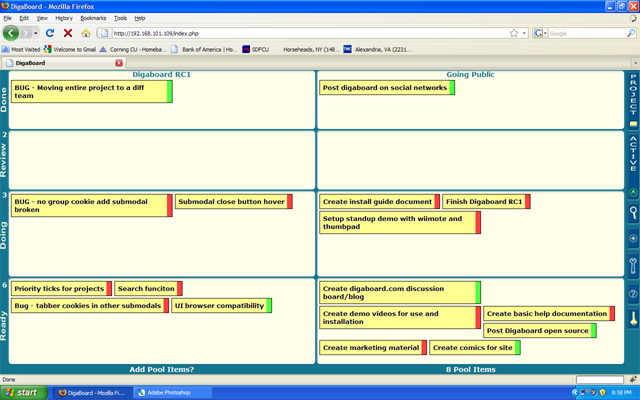
\includegraphics[width=1.0\textwidth]{images/project_board.png}
	\caption{Digaboard Anzeigetafel}
	\label{fig:digaboard}
\end{figure}

Mit dieser Anzeigetafel lassen sich folgende Projektmanagementaufgaben realisieren:
\begin{itemize}
\item Produktanforderungsverwaltung\\
Ein Produkt kann in mehrere Projekte aufgeteilt werden, wobei jedes Projekt seine eigene Spalte in der Anzeigetafel bekommt. Die Anzeigetafel hat mehrere Zeilen, die den Status des Projekts intuitiv darstellen.

\item Task-Planung\\
Die Task-Planung in \emph{Digaboard} ist sehr simpel gehalten. Die Tasks können in der Projekttafel erstellt und einer Zeile zugeordnet werden. Die Zeilen beschreiben den Zustand des Tasks, wie zum Beispiel Ready, Doing, Review und Done. Des Weiteren können hier Fehler eingepflegt werden, die noch zu beseitigen sind.

\item Projektüberwachung\\
Die Projektüberwachung wird durch die übersichtliche Darstellung des Gesamtprozesses auf der Anzeigetafel ermöglicht. Hier können Zeitverzüge bei Tasks leicht erkannt werden.

\item Teamverwaltung\\
Jedes Entwicklerteam bekommt seine eigene Spalte auf der Entwickleranzeigetafel. Dort kann jeder Entwickler seine Taskqueue verwalten.
\end{itemize}

\emph{Digaboard} dient hauptsächlich als Ersatz einer realen Tafel auf der sonst das Projekt dargestellt wird. Diese virtuelle Tafel hat den Vorteil, dass jedes Teammitglied seinen aktuellen Arbeitsstatus über die Webanwendung anpassen kann und sich über den aktuellen Stand des Projektes informieren kann. Jedoch ist die Aufwandsverwaltung und die Zeiterfassung nicht integriert und somit lässt sich \emph{Digaboard} eher als eine Ergänzung für die Projektverwaltung ansehen. \cite {bib:digaboard} \\

\item[IceScrum]\hspace*{1em}\\
Das Projektverwaltungswerkzeug \emph{IceScrum} ist eine web-basierte Server\--Anwendung. Die Anwendung lässt sich mittels eines Webbrowsers ansprechen und benutzen. Der Haupteinsatzzweck dieses Open-Source Werkzeugs ist die agile Vorgehensweise \emph{Scrum}. Zudem bietet \emph{IceScrum} noch Methoden der agilen Vorgehensweise \emph{Kanban}.
Dabei unterstützt die Anwendung das \emph{Scrum} Projektmanagement durch folgende Funktionen:
\begin{itemize}
\item Sprint-Planung\\
Die Sprint-Planung ist bei der agilen Vorgehensweise \emph{Scrum} sehr wichtig. Hierbei können Teammitglieder Tasks für einen Sprint erzeugen. Diese Tasks werden auf einem Dashboard dargestellt. Diese Tasks auf dem Dashboard können dann von Teammitgliedern ausgesucht, begonnen und fertiggestellt werden.

\item Release-Planung\\
Die Planung von Releases erfolgt anhand der Anlegung von Sprints. Innerhalb dieser Sprints werden dann User Stories abgearbeitet. Die Releases werden mit Hilfe der geplanten Sprints und der Teamgröße ermittelt.

\item Produktanforderungsverwaltung\\
Mit Hilfe der Produktanforderungsverwaltung lässt sich die Priorisierung von User Stories durch den Produkt Owner managen.

\item Zeiterfassung\\
Die Zeiterfassung ermöglicht die detaillierte Anzeige von aktuellen Ständen bei Sprints und Releases für jedes Projektmitglied.

\item Projektüberwachung\\
Die Projektüberwachung wird in \emph{IceScrum} durch verschiedene Diagramme wie Burndown, Burnup, Parking Lot und verschiedenen Flussdiagrammen realisiert.

\item Dashboard\\
Das Dashboard ist ein zentraler Bestandteil für den Informationsaustausch. Auf diesem Board sind alle wichtigen Projektinformationen zu finden und auch die letzten Änderungen, Produktvisionen und die Tasks. 
\end{itemize}

Die Entwickler können sich entsprechend ihren Rollen am System einen Account anlegen. So gibt es für jede Projektrolle auch eine dazugehörige Benutzergruppe:
\begin{itemize}
\item Product Owner
\item Scrum Master
\item Stake Holder
\item Developer
\end{itemize}

Des Weiteren bietet \emph{IceScrum} gewisse Funktionen, die aus der \emph{Kanban} Vorgehensweise hervorgehen. Es ist beispielsweise das 'Work in process limit' in die Sprint-Planung mit integriert. \cite{bib:icescrum} \\


\item[XPlanner]\hspace*{1em}\\
Das Open-Source Projekt \emph{XPlanner} hat es sich zur Aufgabe gemacht, die Verwaltung von \emph{XP (Extreme Programming)} Projekten zu unterstützen. \emph{XPlanner} ist ebenfalls ein web-basiertes Werkzeug, dass über einen Webbrowser bedient werden kann. Dabei werden die Methoden des \emph{Extreme Programming} durch folgende Features unterstützt:
\begin{itemize}
\item Planung von User Stories\\
Die Planung von User Stories wird zusammen mit dem Kunden durchgeführt. Der Kunde kann seine gewünschten Funktionalitäten für die nächste Iteration eintragen. Diese Kundenwünsche werden durch den Iteration Manager in Tasks aufgeteilt. Diese Tasks können dann von den Entwicklern in der Iteration abgearbeitet werden.

\item Zeitaufwandserfassung\\
Die Aufwandserfassung ermöglicht den zeitlichen Verlauf von Tasks und User Stories zu ermitteln und auszuwerten. 

\item Entwicklungsprozesse Überwachen\\
Mit \emph{XPlanner} lassen sich sämtliche Tasks, User Stories und Iterationen überwachen. Die Entwicklungsprozesse können nach Status und Zeitablauf visualisiert werden.

\item Task Bearbeitung\\
Die zu bearbeitenden Tasks pro Iteration können von den Entwicklerpaaren ausgewählt werden. 
\end{itemize}

Die Entwickler werden ebenfalls durch eine Zeitaufwandserfassung unterstützt. Diese Zeitaufwandserfassung ermöglicht den Entwicklern eine leichte Aufwandserfassung der geleisteten Arbeit.

Um eine gute Kommunikation mit dem Kunden zu erreichen, hat dieser auch einen Zugang zu dem Projektverwaltungswerkzeug \emph{XPlanner} und kann wie bereits genannt die Funktionen für die nächsten Iterationen vorgeben, die Fortschritte und den Arbeitsaufwand begutachten. Der Kunde kann zusammen mit den Entwicklern einen Release Plan erstellen. \cite{bib:xplanner}

\end{description}

\subsection{Bewertung}
Die im vorherigen Punkt vorgestellten Werkzeuge werden nun anhand ihres Funktionsumfanges bewertet. Es wird keine Bewertung in Bezug  auf Usability oder Performance vorgenommen.  Dabei werden die funktionalen Anforderungen für eine Verwaltung aus dem Unterpunkt \ref{ssec:anforderungen} als Betrachtungskriterien herangezogen.

\begin{enumerate}
\item Ressourcenverwaltung \label{enum:ress}
\item Rollenverteilung \label{enum:roll}
\item Zeitverwaltung \label{enum:zeit}
\item Aufgabenverteilung \label{enum:aufg}
\item Problemmanagement \label{enum:prob}
\item Releaseplanung \label{enum:rele}
\end{enumerate}

\begin{center}
\begin{tabular}[h]{l|c|c|c|c|c|c}
\textbf{Werkzeuge} & \textbf{\ref{enum:ress}} & \textbf{\ref{enum:roll}} & \textbf{\ref{enum:zeit}} & \textbf{\ref{enum:aufg}} & \textbf{\ref{enum:prob}} & \textbf{\ref{enum:rele}}\\
\hline
in-Step S. E. & ++ & + & - & ++ & O & ++\\
TargetProcess & + & ++ & ++ & ++ & + & +\\
TFS 2010 & ++ & O & + & + & ++ & ++\\
\hline
Agilefant & + & ++ & + & + & - & +\\
Agilo for Scrum & + & ++ & - & - & + & +\\
Diagboard & - & - - & - & ++ & O & - -\\
IceScrum & + & ++ & + & + & - - & +\\
XPlanner & + & ++ & + & + & O & O\\
\end{tabular}
\end{center}

Die Tabelle zeigt, dass der Funktionsumfang von Open-Source Anwendungen für agile Projektverwaltung zwar denen von proprietären Anwendungen unterlegen ist, jedoch müssen sich die quelloffenen Anwendungen nicht verstecken. Einige Open-Source Projektverwaltungen haben den Umfang, der einen Produktiveinsatz erlaubt. Die proprietären Projektverwaltungssoftwaren können durch eine gute Integration in Entwicklungsumgebungen und in Versionierungssysteme punkten. Desweiteren unterstützen sie die Qualitätssicherung durch die Verwaltung von Tests und die leichte Einpflege von gefundenen Fehlern.
